\documentclass[12pt,a4paper]{article}

% --- Packages ---
\usepackage[margin=1in]{geometry}
\usepackage{graphicx}
\usepackage{hyperref}
\usepackage{enumitem}
\usepackage{titlesec}
\usepackage{array}
\usepackage{xcolor}
\usepackage{booktabs}
\usepackage{longtable}
\usepackage{tabularx}
\usepackage{amsmath,amssymb}
\usepackage{siunitx}
\usepackage{multirow}
\usepackage{caption}
\usepackage{subcaption}
\usepackage{float}
\usepackage{listings}
\usepackage[ruled,vlined]{algorithm2e}
\usepackage{tikz}
\usetikzlibrary{arrows.meta,positioning,fit,calc,shapes.misc,shapes.geometric}

% --- Branding ---
\definecolor{brandblue}{RGB}{14,75,140}
\definecolor{brandgreen}{RGB}{25,135,84}
\definecolor{brandgray}{RGB}{90,90,100}
\hypersetup{
  colorlinks=true,
  linkcolor=brandblue,
  citecolor=brandblue,
  urlcolor=brandblue
}

% --- Section style ---
\titleformat{\section}{\color{brandblue}\normalfont\Large\bfseries}{}{0em}{}
\titleformat{\subsection}{\color{brandgreen}\normalfont\large\bfseries}{}{0em}{}
\titleformat{\subsubsection}{\color{brandgray}\normalfont\normalsize\bfseries}{}{0em}{}

% --- Listings (code blocks) ---
\lstset{
  basicstyle=\ttfamily\small,
  breaklines=true,
  frame=single,
  rulecolor=\color{brandgray},
  keywordstyle=\color{brandblue}\bfseries,
  commentstyle=\itshape\color{brandgreen},
  stringstyle=\color{brandblue},
  showstringspaces=false
}

% --- Title ---
\title{\vspace{-2em}\textbf{PropertyScout}\\[0.4em]\large The Complete AI-Powered Property Investment Platform}
\author{White Paper}
\date{\today}

\begin{document}
\maketitle
\begin{center}
\textit{Version 1.0 \quad | \quad Confidential Draft for Early Partners and Reviewers}
\end{center}
\vspace{1em}
\tableofcontents
\newpage

% =========================================================
\section{Executive Summary}
PropertyScout is an AI-first property investment platform that automates the end-to-end workflow of sourcing, underwriting, and monitoring UK residential deals. The system integrates automated scraping, robust data validation, AI-based refurbishment cost estimation from listing photos, rental forecasting, cashflow and ROI modeling, EPC matching, forecasting of value uplift, and report generation (PDF and Excel). It is designed for investors, sourcing agents, and estate agencies seeking faster, more consistent decisions with auditability and repeatability.

This document details the current MVP, planned features, reference architecture, data models, algorithms, evaluation frameworks, regulatory controls, commercialization strategy, and a structured roadmap. The goal is to provide technical and commercial clarity for pilot customers, design partners, and potential investors.

\paragraph{Positioning.} Unlike calculators or point tools, PropertyScout focuses on (i) automation across upstream data capture, (ii) AI-driven analysis with human-in-the-loop validation, and (iii) post-purchase monitoring and alerts—creating a continuous value loop.

\paragraph{Outcome.} Reduced analysis time from hours to minutes; consistent underwriting and documentation; proactive alerts; and the ability to scale to hundreds of deals per analyst per week.

% =========================================================
\section{Problem and Opportunity}
\subsection{Industry Pain Points}
\begin{itemize}[leftmargin=1.5em]
  \item \textbf{Fragmented tooling:} Data sourcing, underwriting, EPC checks, and reporting often require multiple systems and manual reconciliation.
  \item \textbf{Latency and inconsistency:} Human analysis varies widely; many deals are lost due to slow turnarounds or inconsistent assumptions.
  \item \textbf{Lack of monitoring:} After purchase, few tools track remortgage windows, interest-rate impacts, or portfolio KPIs in real time.
  \item \textbf{Regional nuance:} Refurb costs and rents are hyper-local; generic calculators miss local reality.
\end{itemize}

\subsection{Why Now}
\begin{itemize}[leftmargin=1.5em]
  \item \textbf{Mature LLMs and vision models} enable robust extraction and estimation from messy sources (HTML, images).
  \item \textbf{API growth} (EPC, ONS, Land Registry, portal data) improves coverage and freshness.
  \item \textbf{Investor demand} for faster, defensible underwriting and automated sourcing/alerts is rising as yields compress.
\end{itemize}

% =========================================================
\section{Product Overview}
\subsection{Elevator Pitch}
PropertyScout is the ultimate AI-powered investment assistant that ingests a property link, extracts structured data, estimates refurb costs from photos, forecasts rents and values, computes full-stack financials, attaches EPC data, and generates client-ready reports—then continues to monitor and alert post-purchase.

\subsection{Current MVP Capabilities}
\begin{enumerate}[leftmargin=1.5em]
  \item URL input $\rightarrow$ \textbf{scrape \& parse} (price, agent, layout, media, key features).
  \item \textbf{AI refurbishment estimation} from images with room-level breakdowns.
  \item \textbf{Rental estimation} using GPT with postcode comparables.
  \item \textbf{Financial stack:} stamp duty, legal/survey/insurance, management fees, yield \& ROI.
  \item \textbf{Value uplift} via HPI-baseline + AI adjustment.
  \item \textbf{EPC matching} to retrieve rating and details.
  \item \textbf{Reporting:} PDF and Excel export; Slack notification with attachments.
\end{enumerate}

\subsection{Planned Features (Highlights)}
\begin{itemize}[leftmargin=1.5em]
  \item Live portal integrations (Rightmove, Zoopla, auctions) with filters, de-dup, and watchlists.
  \item User-configurable alerting on yields, price drops, new listings.
  \item Post-purchase mortgage optimisation, remortgage timing alerts.
  \item Portfolio dashboard, deal comparisons, and client-shareable views.
  \item Off-market CRM tools (compliant outreach) and letter generation.
\end{itemize}

% =========================================================
\section{User Personas \& Jobs-To-Be-Done}
\subsection{Professional Investor}
\textbf{JTBD:} “Underwrite deals consistently and fast; produce investor-ready packs; monitor portfolio KPIs and remortgage opportunities.”

\subsection{Sourcing Agent}
\textbf{JTBD:} “Scan and qualify many deals daily; package them for buyers with credible numbers; run targeted alerts.”

\subsection{Estate Agency (Partner)}
\textbf{JTBD:} “Provide value-add analytics to buyers; white-label reporting; convert more instructions; evidence-based pricing.”

% =========================================================
\section{System Architecture}
\subsection{High-Level Diagram}
\begin{figure}[H]
\centering
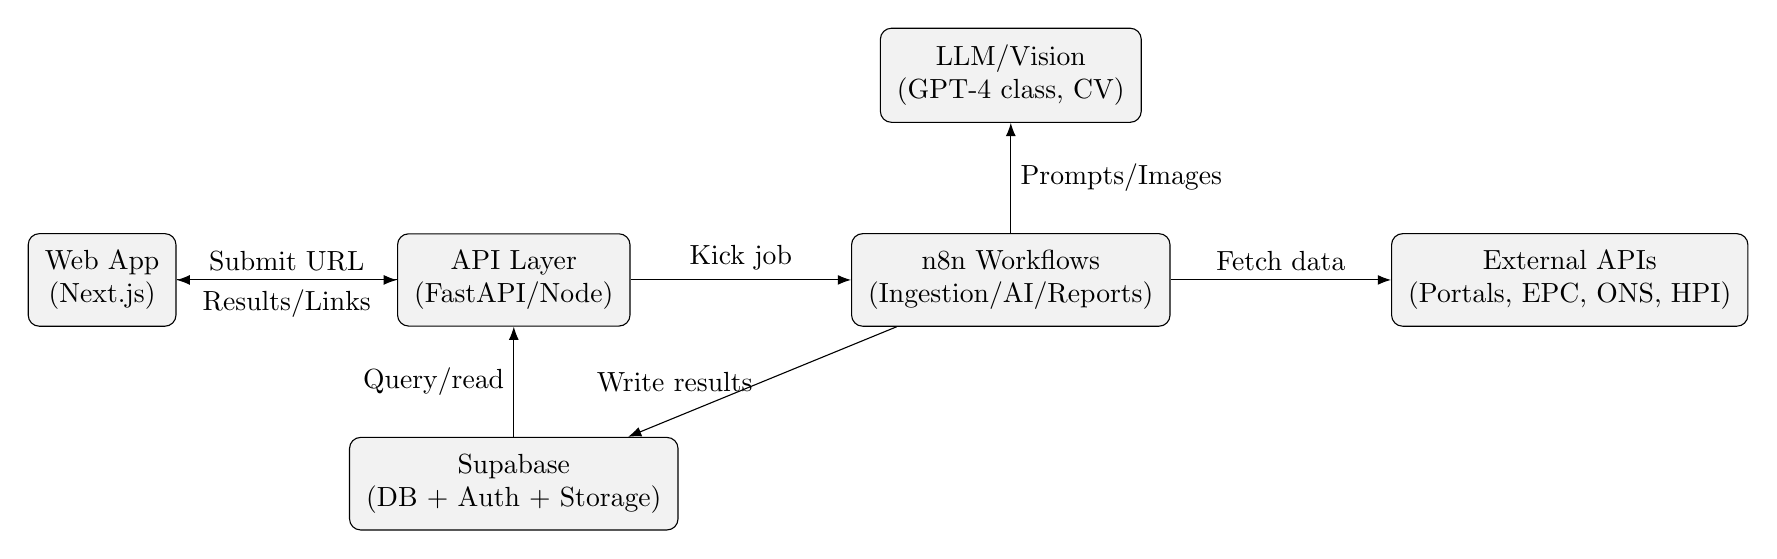
\begin{tikzpicture}[node distance=1.4cm,>=Latex]
\tikzstyle{box}=[draw, rounded corners, align=center, inner sep=6pt]
\node[box, fill=gray!10] (user) {Web App \\ (Next.js)};
\node[box, right=2.8cm of user, fill=gray!10] (api) {API Layer \\ (FastAPI/Node)};
\node[box, right=2.8cm of api, fill=gray!10] (n8n) {n8n Workflows \\ (Ingestion/AI/Reports)};
\node[box, below=1.4cm of api, fill=gray!10] (db) {Supabase \\ (DB + Auth + Storage)};
\node[box, above=1.4cm of n8n, fill=gray!10] (models) {LLM/Vision \\ (GPT-4 class, CV)};
\node[box, right=2.8cm of n8n, fill=gray!10] (ext) {External APIs \\ (Portals, EPC, ONS, HPI)};

\draw[->] (user) -- (api) node[midway, above]{Submit URL};
\draw[->] (api) -- (n8n) node[midway, above]{Kick job};
\draw[->] (n8n) -- (models) node[midway, right]{Prompts/Images};
\draw[->] (n8n) -- (ext) node[midway, above]{Fetch data};
\draw[->] (n8n) -- (db) node[midway, left]{Write results};
\draw[->] (db) -- (api) node[midway, left]{Query/read};
\draw[->] (api) -- (user) node[midway, below]{Results/Links};
\end{tikzpicture}
\caption{PropertyScout high-level architecture.}
\end{figure}

\subsection{Workflow Orchestration (n8n)}
\begin{enumerate}[leftmargin=1.5em]
  \item \textbf{Scrape Node:} Fetch HTML and media links.
  \item \textbf{Clean \& Parse Agent:} Convert HTML to structured JSON (price, address, features).
  \item \textbf{Image Loop:} For each image, run a refurb-estimate prompt, aggregate per room.
  \item \textbf{Rent Agent:} Estimate rent using postcode/regression prior + GPT adjustment.
  \item \textbf{Fees \& ROI Node:} Compute stamp duty, legal, management, net yield, ROI, cashflow.
  \item \textbf{HPI \& Uplift Node:} Calculate baseline uplift; optional AI adjustment.
  \item \textbf{EPC Match Agent:} Find EPC record and extract rating + fields.
  \item \textbf{PDF \& Excel Nodes:} Generate reports; upload to storage.
  \item \textbf{Notify:} Slack/email with links and summary metrics.
\end{enumerate}

\subsection{Data Stores}
\textbf{Supabase:} Postgres for canonical tables (properties, analyses, comps, epc, runs), Storage for PDF/Excel artifacts, Auth for users/teams.

% =========================================================
\section{Data Model (Canonical Schemas)}
\subsection{Core Entities}
\begin{longtable}{@{}p{3.2cm}p{12.4cm}@{}}
\toprule
\textbf{Table} & \textbf{Purpose \& Key Fields} \\
\midrule
\texttt{properties} & Canonical property identity. \textit{Key fields:} id (uuid), url, address\_full, postcode, source, first\_seen, last\_seen, status. \\
\texttt{analyses} & One analysis per run/version. \textit{Key fields:} id, property\_id (fk), run\_timestamp, price, sq\_ft, bedrooms, bathrooms, assumptions jsonb, results jsonb. \\
\texttt{refurb\_estimates} & Room- or item-level refurb costs. \textit{Key fields:} id, analysis\_id (fk), room\_type, items jsonb, subtotal, confidence. \\
\texttt{rent\_estimates} & Rent predictions and sources. \textit{Key fields:} id, analysis\_id (fk), monthly\_rent, method, comps jsonb, confidence. \\
\texttt{fees} & Stamp duty, legal, survey, insurance, mgmt. \textit{Key fields:} id, analysis\_id (fk), duty, legal, survey, insurance, mgmt\_pct, total. \\
\texttt{sales\_comps} & Nearby sales comparables. \textit{Key fields:} id, analysis\_id (fk), address, distance\_m, price, date, sqft, ppsf. \\
\texttt{rental\_comps} & Nearby rental comparables. Fields similar to sales comps. \\
\texttt{epc\_records} & EPC details linked to property. \textit{Key fields:} id, analysis\_id, rating, uprn, lmk\_key, measures jsonb, full\_record jsonb. \\
\texttt{reports} & Generated artifacts. \textit{Key fields:} id, analysis\_id, type (pdf/xlsx), storage\_path, size\_bytes, checksum. \\
\texttt{runs} & Orchestration metadata. \textit{Key fields:} id, user\_id, workflow\_id, duration\_ms, status, error\_log. \\
\bottomrule
\end{longtable}


% =========================================================
\section{Algorithms \& Methods}
\subsection{HTML \texorpdfstring{$\rightarrow$}{->} JSON Extraction}
\textbf{Method:} Heuristic tag selection $+$ LLM cleanup. We use deterministic rules for price/address hints, and an LLM to standardise fields and fill light gaps. Ambiguous fields produce warnings rather than hallucinated values.

\subsection{Vision-Guided Refurb Estimation}
\textbf{Input:} Listing photos; optional captions. \\
\textbf{Process:}
\begin{enumerate}[leftmargin=1.5em]
  \item Image classification: detect room type (kitchen, bathroom, bedroom, lounge, hallway, exterior).
  \item Condition assessment: extract cues (e.g., old cabinets, tile condition, damp marks).
  \item Bill-of-quantities template: map detected items to line-items (e.g., “replace cabinets”, “rewire room”).
  \item Regional cost adjustment: apply postcode-based cost indices.
  \item Confidence scoring: reflect image quality, occlusion, and ambiguity.
\end{enumerate}

\subsection{EPC Matching (Robust Heuristic)}
\textbf{Goal:} From candidate EPC records, select the best match for a given \texttt{propertyTitle} and \texttt{postcode}. \\
\textbf{Steps:}
\begin{enumerate}[leftmargin=1.5em]
  \item Normalise: uppercase; remove punctuation; collapse whitespace.
  \item Extract tokens: house number \& primary street tokens.
  \item Filter by postcode equality (normalised).
  \item Score each record: 
  \[
    s = w_h \cdot \mathbb{1}[\text{house\# match}] + w_s \cdot \text{Jaccard}(street~tokens) - w_e \cdot \text{editDist}(title, address)
  \]
  \item Choose max-$s$; threshold; else null.
\end{enumerate}
Weights $w_h, w_s, w_e$ are tuned from labeled pairs. This approach is fast (linear in candidates) and avoids LLM latency.

\subsection{Rent Estimation}
\textbf{Hybrid model:} Baseline regression using postcode + property features; GPT layer adjusts based on unstructured signals (listing language, amenities, finish quality). Final:
\[
\hat{R} = \alpha \cdot R_{\text{regression}} + (1-\alpha)\cdot R_{\text{GPT}}
\]
with $\alpha$ calibrated by backtesting per region.

\subsection{Fees \& ROI}
Given purchase price $P$, refurb cost $C_r$, other fees $F$, annual rent $R_a$, operating expense ratio $e$, and management fee $\mu$:
\[
\text{NOI} = R_a\cdot(1-e-\mu)
\qquad
\text{Yield} = \frac{\text{NOI}}{P + C_r + F}
\]
For leverage, monthly mortgage $M$ via standard amortisation; monthly cashflow $\text{CF}_m = \frac{\text{NOI}}{12} - M$.

\subsection{Uplift \& Forecasting}
\textbf{Baseline:} Apply HPI growth to $P$; \textbf{Post-refurb uplift} $\Delta$ from comps or AI adjustment; forecast price $P'$:
\[
P' = (P + C_r)\cdot(1 + g_{\text{HPI}}) + \Delta
\]
Sensitivity analysis runs scenarios over $g_{\text{HPI}}$, $R_a$, and $C_r$ with tornado chart outputs (in Excel/PDF).

% =========================================================
\section{Prompts \& Guardrails (Selected)}
\subsection{HTML-to-JSON Prompt (Skeleton)}
\begin{lstlisting}
System: You are a strict data extractor. If a field is unknown, return null.
User: Given raw HTML and images, return ONLY valid JSON with keys:
{price_gbp, address, postcode, bedrooms, bathrooms, tenure, agent, features[]}
Do not invent values. Use best-guess only if explicitly stated by the page.
\end{lstlisting}

\subsection{Refurb Estimation Prompt (Vision)}
\begin{lstlisting}
System: You estimate refurbishment line-items from photos, using UK trade assumptions.
User: For each image, classify room type, list line-items with qty, unit_cost_gbp, subtotal,
and a confidence 0-1. Adjust costs for postcode if provided. Output valid JSON only.
\end{lstlisting}

\subsection{Rent Estimation Prompt}
\begin{lstlisting}
System: You estimate monthly rent in GBP for UK properties.
User: Using the provided structured features and any text cues, output:
{ monthly_rent_gbp, low, high, rationale, confidence }.
Don't exceed local comparables by >15% without specific justification.
\end{lstlisting}

\subsection{EPC Matching Prompt (LLM fallback)}
\begin{lstlisting}
System: You match a single EPC record to a title+postcode and return exactly one JSON object.
User: Inputs: propertyTitle, postcode, epcRecords[]. If unsure, return nulls (no guess).
No markdown. Only JSON.
\end{lstlisting}

% =========================================================
\section{Evaluation \& Accuracy Targets}
\subsection{Metrics}
\begin{itemize}[leftmargin=1.5em]
  \item \textbf{Rent MAE / MAPE:} $| \hat{R} - R |$, percentage error vs. let-agreed rents.
  \item \textbf{Refurb Cost Error:} absolute/relative error vs. post-job invoices or QS estimates.
  \item \textbf{EPC Match Precision/Recall:} on a labeled set.
  \item \textbf{Overall Deal Error:} \% error in Year-1 net yield and cashflow.
\end{itemize}

\subsection{Initial Targets (Beta)}
\begin{itemize}[leftmargin=1.5em]
  \item Rent MAPE: 10–15\% (postcode \& 1–2 bed flats), 15–20\% (mixed stock).
  \item Refurb error: 20–30\% at room-bundle level; 15–25\% with >10 images.
  \item EPC matching: $>$95\% precision on clean addresses; $>$90\% on messy.
  \item Year-1 net yield error: $\pm 1$–1.5pp for standard BTL scenarios.
\end{itemize}

\subsection{Test Protocol}
\begin{enumerate}[leftmargin=1.5em]
  \item Build hold-out set by region and property type.
  \item Backtest on historical listings with known outcomes (rents, invoices).
  \item Report aggregate and per-region metrics; track drift monthly.
\end{enumerate}

% =========================================================
\section{Security, Compliance, and Data Governance}
\subsection{GDPR}
\begin{itemize}[leftmargin=1.5em]
  \item Lawful basis (Legitimate Interests/Contract) for processing listing data.
  \item Data minimisation: only persist fields needed for analysis/audit.
  \item User consent flows for outreach features (opt-in).
\end{itemize}

\subsection{Credentials}
All secrets stored as environment variables or secret managers. Keys redacted in logs and reports. \textbf{Never embed API keys in code or documents.}

\subsection{PII and Retention}
\begin{itemize}[leftmargin=1.5em]
  \item Default retention: analysis artifacts retained 12 months (configurable).
  \item Right to erasure pipeline; access logging; DPA-ready documentation.
\end{itemize}

% =========================================================
\section{Performance \& Cost}
\subsection{Latency Budgets (MVP)}
\begin{itemize}[leftmargin=1.5em]
  \item End-to-end target: 30–90 seconds per property (depends on image count).
  \item Sub-budgets: HTML parse $<$ 3s; images loop $<$ 40s (10–15 images); EPC/API calls $<$ 5s; PDF/Excel $<$ 7s.
\end{itemize}

\subsection{Run Cost (Illustrative)}
\begin{itemize}[leftmargin=1.5em]
  \item LLM tokens (parse + images + rents + EPC): \pounds0.05–\pounds0.20 per run (model/size dependent).
  \item Storage (PDF/Excel): pennies per artifact.
  \item Overall COGS per run (MVP): \pounds0.10–\pounds0.40 typical.
\end{itemize}

% =========================================================
\section{Commercial Strategy}
\subsection{Pricing}
\begin{itemize}[leftmargin=1.5em]
  \item \textbf{Starter:} \pounds29/mo, 50 runs, pay-as-you-go at \pounds1/run thereafter.
  \item \textbf{Pro:} \pounds99/mo, 300 runs, team seats, alerts, PDF/Excel branding.
  \item \textbf{Team/Agency:} \pounds299+/mo, 1{,}000 runs, SSO, white-label, priority support.
  \item \textbf{Custom Region Builds:} One-off setup \& premium monthly (e.g., North West focus), higher accuracy guarantees in coverage zone.
\end{itemize}

\subsection{GTM}
\begin{itemize}[leftmargin=1.5em]
  \item Beta cohort (10–20 users) with discounted lifetime tiers.
  \item Partnerships with sourcing groups \& agents; co-marketed case studies.
  \item Thought leadership: white papers, accuracy dashboards, regional insights.
\end{itemize}

\subsection{Unit Economics (Indicative)}
\begin{itemize}[leftmargin=1.5em]
  \item Gross margin target: $>$80\% at scale with caching and heuristics replacing some LLM calls.
  \item Key levers: model selection, prompt efficiency, deduped runs, batch scoring, regional model fine-tunes.
\end{itemize}

% =========================================================
\section{Risk Register \& Mitigations}
\begin{longtable}{@{}p{3cm}p{7.5cm}p{4.5cm}@{}}
\toprule
\textbf{Risk} & \textbf{Description} & \textbf{Mitigation} \\
\midrule
Data drift & Rents/refurb costs shift regionally. & Monthly backtests; retrain priors; add user feedback weighting. \\
API fragility & Portal/third-party API changes. & Abstraction layer; fallback scrapers; monitoring \& alerts. \\
LLM variability & Different outputs/version changes. & Strict JSON schema validation; retries; guardrails; caching. \\
Compliance & Outreach \& data usage. & GDPR DPIA; opt-in flows; audit logs; updated DPA. \\
COGS creep & Token costs rise. & Smaller models for easy tasks; heuristic prefilters; batch calls. \\
\bottomrule
\end{longtable}

% =========================================================
\section{Roadmap}
\subsection{6-Week Plan (Detailed)}
\begin{longtable}{@{}p{2cm}p{13.6cm}@{}}
\toprule
\textbf{Week} & \textbf{Objectives} \\
\midrule
1 & n8n + Supabase setup; scraper hardened; HTML$\to$JSON prompt; baseline schemas. \\
2 & Basic dashboard; rent regression prior; parameter toggles; initial Excel layout. \\
3 & E2E tests; Slack/email alerting; PDF polish; EPC matching hardening. \\
4 & Off-market CRM MVP; probate/distressed alerts; basic outreach templates. \\
5 & Post-purchase dashboard (rates feed stub); remortgage alert logic. \\
6 & Stress test; docs; demo kit; beta onboarding; support playbooks. \\
\bottomrule
\end{longtable}

\subsection{Post-MVP (Quarterly Themes)}
\begin{itemize}[leftmargin=1.5em]
  \item \textbf{Q1:} Interest-rate forward curve; prompt-tuning pipeline; API quotas \& scaling.
  \item \textbf{Q2:} Regional fine-tunes; deeper comps; A/B of hybrid rent models.
  \item \textbf{Q3:} White-label; embeddable widgets; team workflows.
  \item \textbf{Q4:} Advanced portfolio analytics; acquisition-readiness hardening.
\end{itemize}

% =========================================================
\section{Case Study (Illustrative)}
\subsection{Deal Summary}
\begin{itemize}[leftmargin=1.5em]
  \item Guide price: \pounds525k; 2-bed flat; W2 postcode.
  \item Refurb from images: kitchen refresh, bathroom mid-grade, redecoration.
  \item Rent estimate: \pounds2{,}650/mo (low \pounds2{,}450, high \pounds2{,}850).
\end{itemize}

\subsection{Outputs}
\begin{itemize}[leftmargin=1.5em]
  \item Year-1 net yield: 4.9\% (no leverage); ROI (with leverage): 6.8\%.
  \item Uplift post-refurb: +\SI{6.5}{\percent} baseline; EPC: C (recommended measures: glazing).
  \item PDF generated with breakdown; Slack alert to buyer and agent.
\end{itemize}

% =========================================================
\section{Support, SLAs, and Operations}
\subsection{Beta Support}
\begin{itemize}[leftmargin=1.5em]
  \item Email/Slack within 24h; incident comms; weekly build notes.
  \item Feedback capture in-product; accuracy scorecards per user.
\end{itemize}

\subsection{SLA Targets (Post-Beta)}
\begin{itemize}[leftmargin=1.5em]
  \item 99.5\% uptime monthly; P1 incidents $<$ 4h to mitigate; P2 $<$ 1 business day.
\end{itemize}

% =========================================================
\section{Conclusion}
PropertyScout delivers a practical, automation-first approach to deal analysis: fast ingestion, structured outputs, transparent assumptions, and continuous monitoring. The roadmap emphasizes accuracy, compliance, and operational reliability. With disciplined execution, the platform can become a category-defining operating system for UK residential investors and partners.

% =========================================================
\appendix
\section*{Appendix A: Supabase SQL DDL (Selected)}
\addcontentsline{toc}{section}{Appendix A: Supabase SQL DDL (Selected)}
\begin{lstlisting}[language=SQL]
-- Note: replace schema and tighten types/constraints per environment.
create table public.properties (
  id uuid primary key default gen_random_uuid(),
  url text not null,
  address_full text,
  postcode text,
  source text,
  first_seen timestamptz default now(),
  last_seen timestamptz default now(),
  status text default 'active'
);

create table public.analyses (
  id uuid primary key default gen_random_uuid(),
  property_id uuid references public.properties(id) on delete cascade,
  run_timestamp timestamptz default now(),
  price numeric,
  sq_ft numeric,
  bedrooms int,
  bathrooms int,
  assumptions jsonb not null default '{}',
  results jsonb not null default '{}'
);

create table public.refurb_estimates (
  id uuid primary key default gen_random_uuid(),
  analysis_id uuid references public.analyses(id) on delete cascade,
  room_type text,
  items jsonb not null,
  subtotal numeric,
  confidence numeric
);

create table public.rent_estimates (
  id uuid primary key default gen_random_uuid(),
  analysis_id uuid references public.analyses(id) on delete cascade,
  monthly_rent numeric,
  method text,
  comps jsonb,
  confidence numeric
);

create table public.epc_records (
  id uuid primary key default gen_random_uuid(),
  analysis_id uuid references public.analyses(id) on delete cascade,
  rating text,
  uprn text,
  lmk_key text,
  measures jsonb,
  full_record jsonb
);

create table public.reports (
  id uuid primary key default gen_random_uuid(),
  analysis_id uuid references public.analyses(id) on delete cascade,
  type text check (type in ('pdf','xlsx')),
  storage_path text not null,
  size_bytes bigint,
  checksum text,
  created_at timestamptz default now()
);
\end{lstlisting}

\section*{Appendix B: n8n Workflow (Pseudo-YAML)}
\addcontentsline{toc}{section}{Appendix B: n8n Workflow (Pseudo-YAML)}
\begin{lstlisting}
nodes:
  - Webhook: trigger { url, userId }
  - HTTP: fetch HTML
  - Agent: clean HTML -> JSON (price, address, features)
  - Loop: images[]
      - Agent: refurb estimate per image
  - Code: aggregate refurb lines -> totals
  - Agent: rent estimate (postcodes + comps)
  - Code: fees, stamp duty, management, ROI
  - HTTP: HPI fetch -> uplift baseline
  - HTTP: EPC API -> candidate records
  - Agent: EPC match -> rating + record
  - PDF: compose report
  - Excel: compose spreadsheet
  - Supabase: upsert all tables
  - Slack: send summary + links
\end{lstlisting}

\section*{Appendix C: Report Structure (PDF/Excel)}
\addcontentsline{toc}{section}{Appendix C: Report Structure (PDF/Excel)}
\textbf{PDF Sections:} Cover $\rightarrow$ Summary KPIs $\rightarrow$ Financials $\rightarrow$ Refurb lines $\rightarrow$ Rent \& comps $\rightarrow$ EPC $\rightarrow$ Forecasts $\rightarrow$ Disclaimers. \\
\textbf{Excel Tabs:} Summary, Inputs, Refurb, Rent, Fees, EPC, Forecasts, Comps, Audit.

\section*{Appendix D: API Stubs (FastAPI)}
\addcontentsline{toc}{section}{Appendix D: API Stubs (FastAPI)}
\begin{lstlisting}[language=Python]
from fastapi import FastAPI, HTTPException
from pydantic import BaseModel
import uuid

app = FastAPI()

class RunRequest(BaseModel):
    url: str
    user_id: str

class RunResponse(BaseModel):
    job_id: str
    status: str

@app.post("/analyze", response_model=RunResponse)
def analyze(req: RunRequest):
    job_id = str(uuid.uuid4())
    # enqueue n8n webhook here
    return RunResponse(job_id=job_id, status="queued")
\end{lstlisting}

\section*{Appendix E: Prompt Library (Copy-Paste Ready)}
\addcontentsline{toc}{section}{Appendix E: Prompt Library (Copy-Paste Ready)}
\subsection*{Strict JSON Output Guard}
\begin{lstlisting}
System: Output only VALID JSON. No markdown, no comments. If unsure, use null.
If any schema key is missing, add it with null.
\end{lstlisting}

\subsection*{EPC Match (Final)}
\begin{lstlisting}
System: You are a deterministic matcher. Do not guess.
User: Inputs: { "propertyTitle": "...", "postcode": "...", "epcRecords": [...] }
Rules: normalise strings; exact postcode match required; penalise house-number mismatch;
if none cross a confidence threshold, return matched_epc: null, epc_rating: null.
Output schema:
{
  "property_title": "...",
  "postcode": "...",
  "matched_epc": { ... } | null,
  "epc_rating": "A"|"B"|...|null
}
\end{lstlisting}

\section*{Appendix F: Glossary}
\addcontentsline{toc}{section}{Appendix F: Glossary}
\begin{itemize}[leftmargin=1.5em]
  \item \textbf{EPC:} Energy Performance Certificate.
  \item \textbf{HPI:} House Price Index.
  \item \textbf{NOI:} Net Operating Income.
  \item \textbf{MAPE:} Mean Absolute Percentage Error.
\end{itemize}

\end{document}
